
\documentclass[a4paper,10pt]{scrartcl}

\usepackage[utf8]{inputenc}
\usepackage{tikz}
\usepackage{structuralanalysis}
\usepackage{3dstructuralanalysis}
\usepackage{amsmath}
\usepackage{hyperref}

\usepackage{subfig}
\usepackage{graphicx}
\usepackage{pgfplots}
\usepackage{pgfplotstable}
\tikzset{>=stealth}
\usetikzlibrary{patterns}
\usetikzlibrary{pgfplots.statistics}

\setlength{\paperheight}{30cm}
\setlength{\textheight}{24.5cm}
\setlength{\paperwidth}{21cm}
\setlength{\textwidth}{16.8cm}
\setlength{\oddsidemargin}{-0.3cm}
\setlength{\evensidemargin}{-0.3cm}
\setlength{\parindent}{0cm}
\setlength{\topmargin}{-1.9cm}
\setlength{\headsep}{1.3cm}
\setlength{\footskip}{1.5cm}

\title{Mechanical model of highline forces in case of a helicopter based rescue}

\author{Version 1.0 by Jakob Bludau and Aaron Benkert}



\begin{document}
\maketitle

\section{Mechanical highline model}
The highline will be modeled without explicit details of the anchors. Both anchors are assumed to be fixed points on opposing walls at the same hight and can not transfer moments into the walls. As the backup line is not load bearing in normal conditions it will not be included.

\subsection{No friction, athlete in center}
From general observation there exists a region around the midpoint of the highline where a hanging athlete is not sliding towards the middle while hanging from the leashring after a fall. As the stick friction coefficient is higher than the slip friction coefficient the assumption that the highliner does not slide further without a considerable force being applied seems valid.
For the mechanical model this friction force is problematic, as its value can range from 0 up to $F_A*\nu$. In order to get around this problem, a mechanical model with no friction between leashring and line is considered. In this model, the athlete will always slide to the middle of the highline after a leashfall which is depicted in Fig. \ref{fig::2d::highline::noFric}.

\begin{figure}[ht]
\centering
\begin{tikzpicture}
	\scaling{.65};
	
	
	\point{cosy}{0}{-4};	
	\point{Wall_Left}{0}{0};
	\point{Wall_Right}{20}{0};
	\point{Leash_Ring}{10}{-4};
	\point{Leash_Ring_Projection}{10}{0};
	\point{Harness}{10}{-6};
	

	
	\daxis{1}{cosy}; 
			
	\beam{2}{Wall_Left}{Leash_Ring};
	\beam{2}{Leash_Ring}{Wall_Right};
	\beam{3}{Wall_Left}{Wall_Right};
	\beam{2}{Leash_Ring}{Harness};
	
	\support{1}{Wall_Left}[270];
	\support{1}{Wall_Right}[90];
	
	\hinge{1}{Wall_Left};
	\hinge{1}{Wall_Right};
	\hinge{1}{Leash_Ring};
	

	\node[draw] at (6.55,-4.12)   (a) {$m_A$};
	
	\addon{3}{Wall_Left}{Wall_Right}{Leash_Ring}[0];
	\addon{3}{Wall_Right}{Wall_Left}{Leash_Ring}[-1];
	
	\notation{1}{Wall_Left}{$\alpha$}[xshift=8mm, yshift=-2mm];
	\notation{1}{Wall_Right}{$\alpha$}[xshift=-12mm, yshift=-2mm];
	

	\dimensioning{1}{Wall_Left}{Wall_Right}{+2.0}[$l_0$];
	\dimensioning{1}{Wall_Left}{Leash_Ring_Projection}{+1.0}[$0.5*l_0$];
	\dimensioning{1}{Leash_Ring_Projection}{Wall_Right}{+1.0}[$0.5*l_0$];
	\dimensioning{2}{Leash_Ring_Projection}{Leash_Ring}{+6}[$d$];
	\dimensioning{3}{Wall_Left}{Leash_Ring}{-0.5}[$0.5*s$];
	
\end{tikzpicture}
\caption{Mechanical base model of a loaded highline after a leashfall. There is no friction between the leashring and the highline. The highline spans a gap of length $l_0$. The athlete is represented by the mass $m_A$, the line mass is neglected. The weight of the athlete creates a slack of $d$ in the highline. Backup not shown as it is not load bearing in normal conditions.}
\label{fig::2d::highline::noFric}
\end{figure}

In this simplified case, the model is symmetric and thus simpler to solve. The following independent equations can be formed:

\begin{align*}
tan(\alpha) &= \frac{d}{0.5l_0} \\
F_A &= 2*sin(\alpha)*F_{Line}\\
s &= l_0*(1+(F_{Line}-F_{Preload})/E) 
\end{align*}

With $s$ being the total length the line when it is loaded with the athlete and $E$ being the linearized modulus around the working point (depending on the material and preload that is put onto the line).
For a line with a length of $l_0=60m$ and polyamide ($E=30 kN$) for an athlete with $F_A=80kg*9.81\frac{N}{kg}$, the lineload is $F_{Line}=2.01 kN$. This calculation used a  $F_{Preload}=1.5kN$.

\subsection{No friction, athlete out of center}
From this calculation it becomes obvious, that even if the friction coefficient would be as high as $\nu=0.5$ the resulting force on the line due to friction is negligible compared to the load that is produced by preloading and an athlete hanging in the line. Nevertheless, for the discussion of the contact force with the helicopter hoist cable we want to extend the model to the athlete hanging in other positions than the middle of the highline. Thus (with the knowledge of the above abstraction), we assume that the athlete is hanging in any general position in the highline without sliding into the middle (aka. a mysterious force keeps the body from sliding but the weight is still transferred by the line to the anchors. This results is the line being equally loaded left and right of the leashring. The mechanical 2D base model is shown in Fig. \ref{fig::2d::highline};

\begin{figure}[ht]
\centering
\begin{tikzpicture}
	\scaling{.65};
	
	
	\point{cosy}{0}{-4};	
	\point{Wall_Left}{0}{0};
	\point{Wall_Right}{20}{0};
	\point{Leash_Ring}{8}{-4};
	\point{Leash_Ring_Projection}{8}{0};
	\point{Harness}{8}{-6};
	

	
	\daxis{1}{cosy}; 
			
	\beam{2}{Wall_Left}{Leash_Ring};
	\beam{2}{Leash_Ring}{Wall_Right};
	\beam{3}{Wall_Left}{Wall_Right};
	\beam{2}{Leash_Ring}{Harness};
	
	\support{1}{Wall_Left}[270];
	\support{1}{Wall_Right}[90];
	
	\hinge{1}{Wall_Left};
	\hinge{1}{Wall_Right};
	\hinge{1}{Leash_Ring};
	

	\node[draw] at (5.25,-4.12)   (a) {$m_A$};
	
	\addon{3}{Wall_Left}{Wall_Right}{Leash_Ring}[0];
	\addon{3}{Wall_Right}{Wall_Left}{Leash_Ring}[-1];
	
	\notation{1}{Wall_Left}{$\alpha_L$}[xshift=8mm, yshift=-2mm];
	\notation{1}{Wall_Right}{$\alpha_R$}[xshift=-12mm, yshift=-2mm];
	

	\dimensioning{1}{Wall_Left}{Wall_Right}{+2.0}[$l_0$];
	\dimensioning{1}{Wall_Left}{Leash_Ring_Projection}{+1.0}[$l_L$];
	\dimensioning{1}{Leash_Ring_Projection}{Wall_Right}{+1.0}[$l_R$];
	\dimensioning{2}{Leash_Ring_Projection}{Leash_Ring}{+6}[$d$];
	
	\dimensioning{3}{Wall_Left}{Leash_Ring}{-0.5}[$s_L$];
	\dimensioning{3}{Wall_Right}{Leash_Ring}{0.5}[$s_L$];
	
\end{tikzpicture}
\caption{Mechanical base model of a loaded highline after a leashfall. The highline spans a gap of length $l_0$. The athlete is represented by the mass $m_A$, the line mass is neglected. The weight of the athlete creates a slack of $d$ in the highline. Backup not shown as it is not load bearing in normal conditions.}
\label{fig::2d::highline}
\end{figure}

To declare the forces in the line and leash, the area around the leashring is cut free. The resulting forces are shown in Fig. \ref{fig::2d::forces}.

\begin{figure}[ht]
\centering
\begin{tikzpicture}
	\scaling{.65};
	
	\point{center}{0}{0}
	\point{leash_cut}{0}{-1}
	\point{wall_left}{-2*0.447}{0.447}
	\point{wall_right}{3*0.316}{0.316}
	
	
	\beam{2}{wall_left}{center};
	\beam{2}{wall_right}{center};
	\beam{2}{leash_cut}{center};
	
	\hinge{1}{center};
	
	\load{1}{leash_cut}[90][1.0][-1.1];
	\load{1}{wall_right}[18.44][-1.0][1.1];
	\load{1}{wall_left}[-26.57][1.0][-1.1];
	
	\notation{1}{wall_left}{$F_L$}[xshift=-8mm, yshift=0mm];
	\notation{1}{wall_right}{$F_R$}[xshift=8mm, yshift=-2mm];
	\notation{1}{leash_cut}{$F_A=m_A*g$}[xshift=10mm, yshift=-6mm];

	
\end{tikzpicture}
\caption{Mechanical forces at the area cut around the leashring. The weight force of the athlete $F_A$ is the weight $m_A$ times the gravitational constant $g$. Note, that the two sides of the line are equally loaded but do point in different angles.}
\label{fig::2d::forces}
\end{figure}

In this case there are the following $7$ independent equations that can be formed (given in vector notation):
\begin{align}
tan(\alpha_L) &= \frac{d}{l_L} \\
tan(\alpha_R) &= \frac{d}{l_R} \\
s &= l_0*(1+(F_{Line}-F_{Preload})/E) \\
s &= s_{R}+s_{L} \\
F_A &= F_{Line} (\frac{d}{s_{L}} + \frac{d}{s_{R}}) \\
cos(\alpha_L) &= \frac{l_L}{s_{L}} \\
cos(\alpha_R) &= \frac{l_R}{s_{R}}
\end{align}
This system of equations has $7$ unknowns: $\alpha_L$, $\alpha_R$, $d$, $s$, $s_{R}$, $s_{L}$, $F_{Line}$. As it is well defined, it can be solved with any Newton-Krylov method. Nevertheless, a Levenberg-Marquart solver was $\approx 10^9$ times faster.

\subsection{Restriction of athlete position}

With the model shown in the last section, the angles $\alpha_L$ and $\alpha_R$ can be calculated. Figure \ref{fig::2d::alpha_L} shows the difference of the left and right angle for an athlete with $m=60kg$.

\begin{figure}[ht]
%	\vspace*{-3mm}
\centering
\begin{tikzpicture}
	\begin{axis}[
	name=picture0_0,
	%title=Boundary layer velocity profile,
	ylabel={$\alpha_L-\alpha_R [deg]$},
	xlabel={$\frac{l_L}{l_0}[-]$},
	width=0.5\textwidth,
	grid=major,
%	xmin=0,
%	xmax=1,
	%ymin=-0.0000005,
	%ymax=800,
	%samples=50
	%ytikslabels{,,}
	%height=0.5\textwidth
	] 	
	
	\addplot[mark=none,color={black}] table [x expr={\thisrowno{0}}, y expr={\thisrowno{1}-\thisrowno{2}}, col sep=comma]			{./data/alpha_L.dat};

	\end{axis}
\end{tikzpicture}
\caption{Angle difference for various positions of a $m=60kg$ athlete. Positions are given as ratio $l_L / l_0$}
\label{fig::2d::alpha_L}
\end{figure}

From experience, the leas ring will slide towards the middle if the angle difference  above $\approx 10 deg$. Thus the region below $l < 0.2 l_0$ of either side of the line is excluded from the discussion. As the highline is symmetric with respect to the middle, this holds for both sides.

\section{Highline in contact with helicopter hoist cable}

In the case of a contact between hoist cable and highline the mechanics get more complicated. The main factor is the distance $h_y$ the helicopter is "overflying" the highline. Figure \ref{fig::3d::heli} sketches the situation. The dashed lines represent the reference position. In this case the helicopter is hovering precisely above the middle of the highline. In this reference configuration, the hoist cable is barely touching the highline. If the helicopter "overflies" the highline by moving further in $y$-direction, the hoist cable and highline will be in contact. This situation is sketched in full black lines. 
\setcoords{-25}{10}[1][1.2] 
\setaxis{2} 
%\showpoint 
\begin{figure}[ht]
\centering

\begin{tikzpicture}[coords] 

\dpoint{cosy}{0}{0}{-4};
\dpoint{Wall_Left}{0}{0}{0};
\dpoint{Wall_Right}{15}{0}{0};
\dpoint{Leash_Ring_0}{5}{0}{-4};
\dpoint{Leash_Ring_1}{5}{1}{-3.5};
\dpoint{Leash_Ring_projection_1}{5}{1}{-4};

\dpoint{heli_0}{5}{0}{5};
\dpoint{heli_1}{5}{2}{5};

\dpoint{rescue_0}{5}{0}{-6};
\dpoint{rescue_1}{5}{1}{-6};

\daxis{1}{cosy}

\dsupport{1}{Wall_Left};
\dsupport{1}{Wall_Right};

\dsupport{1}{heli_0};
\dsupport{1}{heli_1};

% loaded line
\dbeam{1}{Wall_Left}{Leash_Ring_1};
\dbeam{1}{Wall_Right}{Leash_Ring_1};

%unloaded liine
\dbeam{3}{Wall_Left}{Leash_Ring_0};
\dbeam{3}{Wall_Right}{Leash_Ring_0};

%unloaded heli
\dbeam{3}{heli_0}{rescue_0};

%loaded heli
\dbeam{1}{heli_1}{Leash_Ring_1};
\dbeam{1}{rescue_1}{Leash_Ring_1};

\dhinge{1}{Wall_Left};
\dhinge{1}{Wall_Right};
\dhinge{1}{Leash_Ring_1};
\dhinge{1}{heli_0};
\dhinge{1}{heli_1};

%highline cable contact patch
\ddimensioning{yx}{Leash_Ring_0}{Leash_Ring_projection_1}{9}[$e_y$][3];
\ddimensioning{zy}{Leash_Ring_1}{Leash_Ring_projection_1}{3}[$e_z$][2.3];

%helicopter overshoot
\ddimensioning{yx}{heli_0}{heli_1}{-0.5}[$h_y$][3.5];

%helicopter height
\ddimensioning{zy}{heli_0}{Leash_Ring_0}{-1.5}[$h_z$][5.5];


%%some helping notations
\dnotation{1}{heli_0}{Helicopter hoist}[xshift=3mm,yshift=12mm];

\dnotation{1}{Wall_Left}{Left anchor}[above right];
\dnotation{1}{Wall_Right}{Right anchor}[above right];
\end{tikzpicture}
\caption{Three-dimensional depiction of the contact between highline and helicopter hoist cable. The helicopter is approaching from the negative $y$ direction. Thus the dashed lines represent the helicopter hovering exactly above the leashring and the rescuer hanging straight down from the hoist. In this case the highline and hoist cable are in unloaded contact. As the helicopter drifts further into the $y$ direction and passes over the line, it creates a load in the contact point between hoist cable and highline. This case is represented by the full lines.}
\label{fig::3d::heli}
\end{figure}

In the following the cases with contact between helicopter hoist cable and highline are discussed. The discussion is restricted to contact at the leash ring. This is assumed to be the worst case, as the leash ring forces the line material to be flat and the contact with the hoist cable will be with the sidewall of the tubular highline material. Because of the construction of highline webbings, this is considered to be the weakpoint for cutting forces.
Figure \ref{fig::2d::highline_hoist} shows the view from the right anchor looking towards the left anchor of figure \ref{fig::3d::heli}.

\begin{figure}[ht]
\centering
\begin{tikzpicture}
	\scaling{.65};
	
	\point{center_0}{0}{0}
	\point{anchor}{0}{4}
	\point{heli_0}{0}{8}
	\point{heli_1}{4}{8}
	\point{rescuer_0}{0}{-2}
	\point{rescuer_1}{2}{-2}
	\point{center_1}{2}{1}
	\point{angle_1}{2}{4}

	
	\beam{3}{heli_0}{rescuer_0};
	\beam{3}{center_1}{angle_1};
	\beam{2}{heli_1}{center_1};
	\beam{2}{center_1}{rescuer_1}
	\beam{2}{anchor}{center_1}
	
	\hinge{1}{center_0};
	\hinge{1}{center_1};
	
	\hinge{1}{heli_0};
	\hinge{1}{heli_1};
	
	\hinge{1}{anchor};
	
	\notation{1}{center_1}{$\beta$}[xshift=2mm, yshift=15mm];
	\notation{1}{anchor}{$\Psi$}[xshift=3mm, yshift=-10mm];
	
	\notation{1}{heli_0}{Helicopter hoist}[xshift=13mm, yshift=5mm];
	
	\notation{1}{anchor}{Left anchor}[xshift=2mm, yshift=5mm];
	
	\dimensioning{1}{center_0}{center_1}{-1.0}[$e_y$];
	\dimensioning{2}{center_0}{center_1}{-0.5}[$e_z$];
	
	\dimensioning{1}{heli_0}{heli_1}{+7.0}[$h_y$];
	\dimensioning{2}{center_0}{heli_1}{-1.0}[$h_z$];

	
\end{tikzpicture}
\caption{Side view from right anchor looking towards left anchor. Dashed lines represent the reference configuration, full lines the situation with mechanical contact between highline and hoist cable}
\label{fig::2d::highline_hoist}
\end{figure}

This case can mechanically be divided into two parts: The highline with non-central athlete including an additional contact force $F_C$ and the helicopter with hoist, cable, and the weight of the rescuer. The forces at the hoist cable are shown in \ref{fig::2d::hoist}.

\begin{figure}[ht]
\centering
\begin{tikzpicture}
	\scaling{.65};
	
	\point{center_0}{0}{0}
	\point{heli_0}{0}{8}
	\point{heli_1}{4}{8}
	\point{rescuer_0}{0}{-2}
	\point{rescuer_1}{2}{-2}
	\point{center_1}{2}{1}
	\point{angle_1}{2}{4}

	
	\beam{3}{heli_0}{rescuer_0};
	\beam{3}{center_1}{angle_1};
	\beam{2}{heli_1}{center_1};
	\beam{2}{center_1}{rescuer_1}
	
	\hinge{1}{center_0};
	\hinge{1}{center_1};
	
	\load{1}{rescuer_0}[90][1.0][-1.1];
	\load{1}{rescuer_1}[90][1.0][-1.1];
	
	\load{1}{heli_0}[270][1.0][-1.1];
	\load{1}{heli_1}[254.05][1.0][-1.1];
	\load{1}{center_1}[0][1.0][-1.1];
	
	\notation{1}{center_1}{$\beta$}[xshift=2mm, yshift=15mm];
	
	\notation{1}{heli_0}{$F_R$}[xshift=-8mm, yshift=5mm];
	\notation{1}{rescuer_0}{$F_R$}[xshift=-8mm, yshift=-5mm];
	
	\notation{1}{heli_1}{$F_H$}[xshift=+8mm, yshift=5mm];
	\notation{1}{rescuer_1}{$F_R$}[xshift=+8mm, yshift=-5mm];
	\notation{1}{center_1}{$F_C$}[xshift=-5mm, yshift=5mm];
	
	\dimensioning{1}{center_0}{center_1}{-1.0}[$e_y$];
	\dimensioning{2}{center_0}{center_1}{-0.5}[$e_z$];
	
	\dimensioning{1}{heli_0}{heli_1}{+7.0}[$h_y$];
	\dimensioning{2}{center_0}{heli_1}{-1.0}[$h_z$];

	
\end{tikzpicture}
\caption{Mechanical forces at the isolated hoist cable. View along main highline direction. Dashed lines represent the reference state where line and cable begin to touch. $F_C$ is the force in the contact point with the highline. $F_R$ is the weight force of the rescuer, $F_H$ the cable transfers onto the helicopter.}
\label{fig::2d::hoist}
\end{figure}

From the geometric conditions shown in \ref{fig::2d::hoist}, the following minimal set of independent equations can be derived:
\begin{align*}
tan(\beta) &= \frac{h_{y}-e_y}{h_z-e_z} \\
sin(\beta) F_H &= F_C \\
cos(\beta) F_H &= m_R*g
\end{align*}

As this set of 3 equations contains the 3 unknowns $F_C$, $e_z$, and $e_y$. Nevertheless, $e_z$ and $e_y$ can be expressed as functions of $\Psi$ and already defined unknowns from the highline mechanics. Figure \ref{fig::2d::highline_side} gives an overview of the mechanics.

\begin{figure}[ht]
\centering
\begin{tikzpicture}
	\scaling{.65};
	
	\point{center_0}{0}{0}
	\point{anchor}{0}{4}
	\point{heli_0}{0}{8}
	\point{rescuer_0}{0}{-2}
	\point{rescuer_1}{2}{-2}
	\point{center_1}{2}{1}


	
	\beam{3}{heli_0}{rescuer_0};
	\beam{2}{center_1}{rescuer_1}
	\beam{2}{anchor}{center_1}
	
	\hinge{1}{center_0};
	\hinge{1}{center_1};
	
	\hinge{1}{heli_0};
	
	\hinge{1}{anchor};
	
	\load{1}{center_1}[180][1.0][-1.1];
	\load{1}{rescuer_1}[90][1.0][-1.1];
	
	\notation{1}{anchor}{$\Psi$}[xshift=3mm, yshift=-10mm];
	
	\notation{1}{heli_0}{Helicopter hoist}[xshift=13mm, yshift=5mm];
	
	\notation{1}{anchor}{Left anchor}[xshift=2mm, yshift=5mm];
	
	\notation{1}{rescuer_1}{$F_A$}[xshift=+8mm, yshift=-5mm];
	\notation{1}{center_1}{$F_C$}[xshift=+5mm, yshift=5mm];
	
	\dimensioning{1}{center_0}{center_1}{-1.0}[$e_y$];
	\dimensioning{2}{center_0}{center_1}{-0.5}[$e_z$];
	
	\dimensioning{3}{anchor}{center_1}{+0.25}[$d$];

	
\end{tikzpicture}
\caption{Side view from right anchor looking towards left anchor. Dashed lines represent the reference configuration of the hoist cable. Full lines represent the highline loaded with the contact force $F_C$, pulled by $\Psi$ towards the $y$-direction.}
\label{fig::2d::highline_side}
\end{figure}

From the geometry in this view the following equations relating $\Psi$ with $e_z$ and $e_y$ can be derived:
\begin{align*}
\sin(\Psi) d &= e_y \\
d(1-cos(\Psi)) &= e_z \\
tan(\Psi) &=\frac{F_C}{F_A}
\end{align*}
With the equation for $\Psi$, the mechanical system of the hoist and highline can be connected into one system with 11 equations and unknowns. As the mechanics of the highline is rotatory symmetric in the $x$-axis, the force acting on the highline is $F=\sqrt{F_C^2+F_A^2}$. The rest of the highline mechanics stays unchanged. 

The used Python code to solve the SoE and produce the plots is available from the authors, just write us.

\section{Resulting mechanical forces}

In the following the results of the mechanical model are presented. Although the model calculates a variety of variables, the contact force $F_C$ is focused. This results from the assumption that the damage the hoist cable can inflict on the highline webbing is strongly dependent on $F_C$. At this time this is clearly marked as an assumption. Results from experiments might not confirm this assumption and even if it is confirmed, there might be other more important factors mediating damage on the webbing by the hoist cable. In the following the most important factors influencing $F_C$ are discussed. The results are separated in helicopter related variables and highline related variables.

\subsection{Highline related variables}
Figure \ref{fig::highline::vars} shows the influence of $l_0$, $m_A$, $l_L/l_0$, and $preTension$ on $F_C$. Furthermore the material 'PinkTube' (Polyamid) is shown in full, 'Y2K' (Dyneema) in dashed lines.  
\begin{figure}[ht]
\centering
% Created by tikzDevice version 0.12.6 on 2024-01-05 10:48:34
% !TEX encoding = UTF-8 Unicode
\begin{tikzpicture}[x=1pt,y=1pt]
\definecolor{fillColor}{RGB}{255,255,255}
\path[use as bounding box,fill=fillColor,fill opacity=0.00] (0,0) rectangle (216.81,216.81);
\begin{scope}
\path[clip] (  0.00,  0.00) rectangle (216.81,216.81);
\definecolor{drawColor}{RGB}{255,255,255}
\definecolor{fillColor}{RGB}{255,255,255}

\path[draw=drawColor,line width= 0.6pt,line join=round,line cap=round,fill=fillColor] (  0.00,  0.00) rectangle (216.81,216.81);
\end{scope}
\begin{scope}
\path[clip] ( 36.11, 30.69) rectangle (211.31,211.31);
\definecolor{fillColor}{RGB}{255,255,255}

\path[fill=fillColor] ( 36.11, 30.69) rectangle (211.31,211.31);
\definecolor{drawColor}{gray}{0.87}

\path[draw=drawColor,line width= 0.1pt,line join=round] ( 36.11, 63.04) --
	(211.31, 63.04);

\path[draw=drawColor,line width= 0.1pt,line join=round] ( 36.11,111.34) --
	(211.31,111.34);

\path[draw=drawColor,line width= 0.1pt,line join=round] ( 36.11,159.63) --
	(211.31,159.63);

\path[draw=drawColor,line width= 0.1pt,line join=round] ( 36.11,207.93) --
	(211.31,207.93);

\path[draw=drawColor,line width= 0.1pt,line join=round] ( 52.68, 30.69) --
	( 52.68,211.31);

\path[draw=drawColor,line width= 0.1pt,line join=round] ( 95.73, 30.69) --
	( 95.73,211.31);

\path[draw=drawColor,line width= 0.1pt,line join=round] (138.78, 30.69) --
	(138.78,211.31);

\path[draw=drawColor,line width= 0.1pt,line join=round] (181.82, 30.69) --
	(181.82,211.31);

\path[draw=drawColor,line width= 0.3pt,line join=round] ( 36.11, 38.90) --
	(211.31, 38.90);

\path[draw=drawColor,line width= 0.3pt,line join=round] ( 36.11, 87.19) --
	(211.31, 87.19);

\path[draw=drawColor,line width= 0.3pt,line join=round] ( 36.11,135.49) --
	(211.31,135.49);

\path[draw=drawColor,line width= 0.3pt,line join=round] ( 36.11,183.78) --
	(211.31,183.78);

\path[draw=drawColor,line width= 0.3pt,line join=round] ( 74.21, 30.69) --
	( 74.21,211.31);

\path[draw=drawColor,line width= 0.3pt,line join=round] (117.25, 30.69) --
	(117.25,211.31);

\path[draw=drawColor,line width= 0.3pt,line join=round] (160.30, 30.69) --
	(160.30,211.31);

\path[draw=drawColor,line width= 0.3pt,line join=round] (203.35, 30.69) --
	(203.35,211.31);
\definecolor{drawColor}{RGB}{0,0,0}

\path[draw=drawColor,line width= 0.6pt,line join=round] ( 44.07,193.76) --
	( 48.38,177.90) --
	( 56.99,151.47) --
	( 65.60,130.35) --
	( 74.21,113.08) --
	( 82.82, 98.71) --
	(100.04, 76.15) --
	(117.25, 59.28);

\path[draw=drawColor,line width= 0.6pt,dash pattern=on 4pt off 4pt ,line join=round] ( 56.99,177.93) --
	( 65.60,158.97) --
	( 74.21,142.71) --
	( 82.82,128.65) --
	(100.04,105.61) --
	(117.25, 87.59) --
	(160.30, 56.11);
\definecolor{drawColor}{gray}{0.70}

\path[draw=drawColor,line width= 0.6pt,line join=round,line cap=round] ( 36.11, 30.69) rectangle (211.31,211.31);
\end{scope}
\begin{scope}
\path[clip] (  0.00,  0.00) rectangle (216.81,216.81);
\definecolor{drawColor}{gray}{0.30}

\node[text=drawColor,anchor=base east,inner sep=0pt, outer sep=0pt, scale=  0.88] at ( 31.16, 35.87) {100};

\node[text=drawColor,anchor=base east,inner sep=0pt, outer sep=0pt, scale=  0.88] at ( 31.16, 84.16) {150};

\node[text=drawColor,anchor=base east,inner sep=0pt, outer sep=0pt, scale=  0.88] at ( 31.16,132.46) {200};

\node[text=drawColor,anchor=base east,inner sep=0pt, outer sep=0pt, scale=  0.88] at ( 31.16,180.75) {250};
\end{scope}
\begin{scope}
\path[clip] (  0.00,  0.00) rectangle (216.81,216.81);
\definecolor{drawColor}{gray}{0.70}

\path[draw=drawColor,line width= 0.3pt,line join=round] ( 33.36, 38.90) --
	( 36.11, 38.90);

\path[draw=drawColor,line width= 0.3pt,line join=round] ( 33.36, 87.19) --
	( 36.11, 87.19);

\path[draw=drawColor,line width= 0.3pt,line join=round] ( 33.36,135.49) --
	( 36.11,135.49);

\path[draw=drawColor,line width= 0.3pt,line join=round] ( 33.36,183.78) --
	( 36.11,183.78);
\end{scope}
\begin{scope}
\path[clip] (  0.00,  0.00) rectangle (216.81,216.81);
\definecolor{drawColor}{gray}{0.70}

\path[draw=drawColor,line width= 0.3pt,line join=round] ( 74.21, 27.94) --
	( 74.21, 30.69);

\path[draw=drawColor,line width= 0.3pt,line join=round] (117.25, 27.94) --
	(117.25, 30.69);

\path[draw=drawColor,line width= 0.3pt,line join=round] (160.30, 27.94) --
	(160.30, 30.69);

\path[draw=drawColor,line width= 0.3pt,line join=round] (203.35, 27.94) --
	(203.35, 30.69);
\end{scope}
\begin{scope}
\path[clip] (  0.00,  0.00) rectangle (216.81,216.81);
\definecolor{drawColor}{gray}{0.30}

\node[text=drawColor,anchor=base,inner sep=0pt, outer sep=0pt, scale=  0.88] at ( 74.21, 19.68) {100};

\node[text=drawColor,anchor=base,inner sep=0pt, outer sep=0pt, scale=  0.88] at (117.25, 19.68) {200};

\node[text=drawColor,anchor=base,inner sep=0pt, outer sep=0pt, scale=  0.88] at (160.30, 19.68) {300};

\node[text=drawColor,anchor=base,inner sep=0pt, outer sep=0pt, scale=  0.88] at (203.35, 19.68) {400};
\end{scope}
\begin{scope}
\path[clip] (  0.00,  0.00) rectangle (216.81,216.81);
\definecolor{drawColor}{RGB}{0,0,0}

\node[text=drawColor,anchor=base,inner sep=0pt, outer sep=0pt, scale=  1.10] at (123.71,  7.64) {$l_0 [m]$};
\end{scope}
\begin{scope}
\path[clip] (  0.00,  0.00) rectangle (216.81,216.81);
\definecolor{drawColor}{RGB}{0,0,0}

\node[text=drawColor,rotate= 90.00,anchor=base,inner sep=0pt, outer sep=0pt, scale=  1.10] at ( 13.08,121.00) {$F_C [N]$};
\end{scope}
\end{tikzpicture}
\begin{tikzpicture}[x=1pt,y=1pt]
\definecolor{fillColor}{RGB}{255,255,255}
\path[use as bounding box,fill=fillColor,fill opacity=0.00] (0,0) rectangle (216.81,216.81);
\begin{scope}
\path[clip] (  0.00,  0.00) rectangle (216.81,216.81);
\definecolor{drawColor}{RGB}{255,255,255}
\definecolor{fillColor}{RGB}{255,255,255}

\path[draw=drawColor,line width= 0.6pt,line join=round,line cap=round,fill=fillColor] (  0.00,  0.00) rectangle (216.81,216.81);
\end{scope}
\begin{scope}
\path[clip] ( 36.11, 30.69) rectangle (211.31,211.31);
\definecolor{fillColor}{RGB}{255,255,255}

\path[fill=fillColor] ( 36.11, 30.69) rectangle (211.31,211.31);
\definecolor{drawColor}{gray}{0.87}

\path[draw=drawColor,line width= 0.1pt,line join=round] ( 36.11, 63.04) --
	(211.31, 63.04);

\path[draw=drawColor,line width= 0.1pt,line join=round] ( 36.11,111.34) --
	(211.31,111.34);

\path[draw=drawColor,line width= 0.1pt,line join=round] ( 36.11,159.63) --
	(211.31,159.63);

\path[draw=drawColor,line width= 0.1pt,line join=round] ( 36.11,207.93) --
	(211.31,207.93);

\path[draw=drawColor,line width= 0.1pt,line join=round] ( 70.62, 30.69) --
	( 70.62,211.31);

\path[draw=drawColor,line width= 0.1pt,line join=round] (123.71, 30.69) --
	(123.71,211.31);

\path[draw=drawColor,line width= 0.1pt,line join=round] (176.80, 30.69) --
	(176.80,211.31);

\path[draw=drawColor,line width= 0.3pt,line join=round] ( 36.11, 38.90) --
	(211.31, 38.90);

\path[draw=drawColor,line width= 0.3pt,line join=round] ( 36.11, 87.19) --
	(211.31, 87.19);

\path[draw=drawColor,line width= 0.3pt,line join=round] ( 36.11,135.49) --
	(211.31,135.49);

\path[draw=drawColor,line width= 0.3pt,line join=round] ( 36.11,183.78) --
	(211.31,183.78);

\path[draw=drawColor,line width= 0.3pt,line join=round] ( 44.07, 30.69) --
	( 44.07,211.31);

\path[draw=drawColor,line width= 0.3pt,line join=round] ( 97.17, 30.69) --
	( 97.17,211.31);

\path[draw=drawColor,line width= 0.3pt,line join=round] (150.26, 30.69) --
	(150.26,211.31);

\path[draw=drawColor,line width= 0.3pt,line join=round] (203.35, 30.69) --
	(203.35,211.31);
\definecolor{drawColor}{RGB}{0,0,0}

\path[draw=drawColor,line width= 0.6pt,line join=round] ( 44.07,148.38) --
	( 97.17,151.47) --
	(150.26,154.07) --
	(203.35,156.32);

\path[draw=drawColor,line width= 0.6pt,dash pattern=on 4pt off 4pt ,line join=round] ( 44.07,172.35) --
	( 97.17,177.93) --
	(150.26,182.86) --
	(203.35,187.13);
\definecolor{drawColor}{gray}{0.70}

\path[draw=drawColor,line width= 0.6pt,line join=round,line cap=round] ( 36.11, 30.69) rectangle (211.31,211.31);
\end{scope}
\begin{scope}
\path[clip] (  0.00,  0.00) rectangle (216.81,216.81);
\definecolor{drawColor}{gray}{0.30}

\node[text=drawColor,anchor=base east,inner sep=0pt, outer sep=0pt, scale=  0.88] at ( 31.16, 35.87) {100};

\node[text=drawColor,anchor=base east,inner sep=0pt, outer sep=0pt, scale=  0.88] at ( 31.16, 84.16) {150};

\node[text=drawColor,anchor=base east,inner sep=0pt, outer sep=0pt, scale=  0.88] at ( 31.16,132.46) {200};

\node[text=drawColor,anchor=base east,inner sep=0pt, outer sep=0pt, scale=  0.88] at ( 31.16,180.75) {250};
\end{scope}
\begin{scope}
\path[clip] (  0.00,  0.00) rectangle (216.81,216.81);
\definecolor{drawColor}{gray}{0.70}

\path[draw=drawColor,line width= 0.3pt,line join=round] ( 33.36, 38.90) --
	( 36.11, 38.90);

\path[draw=drawColor,line width= 0.3pt,line join=round] ( 33.36, 87.19) --
	( 36.11, 87.19);

\path[draw=drawColor,line width= 0.3pt,line join=round] ( 33.36,135.49) --
	( 36.11,135.49);

\path[draw=drawColor,line width= 0.3pt,line join=round] ( 33.36,183.78) --
	( 36.11,183.78);
\end{scope}
\begin{scope}
\path[clip] (  0.00,  0.00) rectangle (216.81,216.81);
\definecolor{drawColor}{gray}{0.70}

\path[draw=drawColor,line width= 0.3pt,line join=round] ( 44.07, 27.94) --
	( 44.07, 30.69);

\path[draw=drawColor,line width= 0.3pt,line join=round] ( 97.17, 27.94) --
	( 97.17, 30.69);

\path[draw=drawColor,line width= 0.3pt,line join=round] (150.26, 27.94) --
	(150.26, 30.69);

\path[draw=drawColor,line width= 0.3pt,line join=round] (203.35, 27.94) --
	(203.35, 30.69);
\end{scope}
\begin{scope}
\path[clip] (  0.00,  0.00) rectangle (216.81,216.81);
\definecolor{drawColor}{gray}{0.30}

\node[text=drawColor,anchor=base,inner sep=0pt, outer sep=0pt, scale=  0.88] at ( 44.07, 19.68) {60};

\node[text=drawColor,anchor=base,inner sep=0pt, outer sep=0pt, scale=  0.88] at ( 97.17, 19.68) {80};

\node[text=drawColor,anchor=base,inner sep=0pt, outer sep=0pt, scale=  0.88] at (150.26, 19.68) {100};

\node[text=drawColor,anchor=base,inner sep=0pt, outer sep=0pt, scale=  0.88] at (203.35, 19.68) {120};
\end{scope}
\begin{scope}
\path[clip] (  0.00,  0.00) rectangle (216.81,216.81);
\definecolor{drawColor}{RGB}{0,0,0}

\node[text=drawColor,anchor=base,inner sep=0pt, outer sep=0pt, scale=  1.10] at (123.71,  7.64) {$m_A [kg]$};
\end{scope}
\begin{scope}
\path[clip] (  0.00,  0.00) rectangle (216.81,216.81);
\definecolor{drawColor}{RGB}{0,0,0}

\node[text=drawColor,rotate= 90.00,anchor=base,inner sep=0pt, outer sep=0pt, scale=  1.10] at ( 13.08,121.00) {$F_C [N]$};
\end{scope}
\end{tikzpicture}
\begin{tikzpicture}[x=1pt,y=1pt]
\definecolor{fillColor}{RGB}{255,255,255}
\path[use as bounding box,fill=fillColor,fill opacity=0.00] (0,0) rectangle (216.81,216.81);
\begin{scope}
\path[clip] (  0.00,  0.00) rectangle (216.81,216.81);
\definecolor{drawColor}{RGB}{255,255,255}
\definecolor{fillColor}{RGB}{255,255,255}

\path[draw=drawColor,line width= 0.6pt,line join=round,line cap=round,fill=fillColor] (  0.00,  0.00) rectangle (216.81,216.81);
\end{scope}
\begin{scope}
\path[clip] ( 36.11, 30.69) rectangle (211.31,211.31);
\definecolor{fillColor}{RGB}{255,255,255}

\path[fill=fillColor] ( 36.11, 30.69) rectangle (211.31,211.31);
\definecolor{drawColor}{gray}{0.87}

\path[draw=drawColor,line width= 0.1pt,line join=round] ( 36.11, 63.04) --
	(211.31, 63.04);

\path[draw=drawColor,line width= 0.1pt,line join=round] ( 36.11,111.34) --
	(211.31,111.34);

\path[draw=drawColor,line width= 0.1pt,line join=round] ( 36.11,159.63) --
	(211.31,159.63);

\path[draw=drawColor,line width= 0.1pt,line join=round] ( 36.11,207.93) --
	(211.31,207.93);

\path[draw=drawColor,line width= 0.1pt,line join=round] ( 70.62, 30.69) --
	( 70.62,211.31);

\path[draw=drawColor,line width= 0.1pt,line join=round] (123.71, 30.69) --
	(123.71,211.31);

\path[draw=drawColor,line width= 0.1pt,line join=round] (176.80, 30.69) --
	(176.80,211.31);

\path[draw=drawColor,line width= 0.3pt,line join=round] ( 36.11, 38.90) --
	(211.31, 38.90);

\path[draw=drawColor,line width= 0.3pt,line join=round] ( 36.11, 87.19) --
	(211.31, 87.19);

\path[draw=drawColor,line width= 0.3pt,line join=round] ( 36.11,135.49) --
	(211.31,135.49);

\path[draw=drawColor,line width= 0.3pt,line join=round] ( 36.11,183.78) --
	(211.31,183.78);

\path[draw=drawColor,line width= 0.3pt,line join=round] ( 44.07, 30.69) --
	( 44.07,211.31);

\path[draw=drawColor,line width= 0.3pt,line join=round] ( 97.17, 30.69) --
	( 97.17,211.31);

\path[draw=drawColor,line width= 0.3pt,line join=round] (150.26, 30.69) --
	(150.26,211.31);

\path[draw=drawColor,line width= 0.3pt,line join=round] (203.35, 30.69) --
	(203.35,211.31);
\definecolor{drawColor}{RGB}{0,0,0}

\path[draw=drawColor,line width= 0.6pt,line join=round] ( 44.07,176.75) --
	( 97.17,161.33) --
	(150.26,153.92) --
	(203.35,151.47);

\path[draw=drawColor,line width= 0.6pt,dash pattern=on 4pt off 4pt ,line join=round] ( 44.07,197.63) --
	( 97.17,186.05) --
	(150.26,179.88) --
	(203.35,177.93);
\definecolor{drawColor}{gray}{0.70}

\path[draw=drawColor,line width= 0.6pt,line join=round,line cap=round] ( 36.11, 30.69) rectangle (211.31,211.31);
\end{scope}
\begin{scope}
\path[clip] (  0.00,  0.00) rectangle (216.81,216.81);
\definecolor{drawColor}{gray}{0.30}

\node[text=drawColor,anchor=base east,inner sep=0pt, outer sep=0pt, scale=  0.88] at ( 31.16, 35.87) {100};

\node[text=drawColor,anchor=base east,inner sep=0pt, outer sep=0pt, scale=  0.88] at ( 31.16, 84.16) {150};

\node[text=drawColor,anchor=base east,inner sep=0pt, outer sep=0pt, scale=  0.88] at ( 31.16,132.46) {200};

\node[text=drawColor,anchor=base east,inner sep=0pt, outer sep=0pt, scale=  0.88] at ( 31.16,180.75) {250};
\end{scope}
\begin{scope}
\path[clip] (  0.00,  0.00) rectangle (216.81,216.81);
\definecolor{drawColor}{gray}{0.70}

\path[draw=drawColor,line width= 0.3pt,line join=round] ( 33.36, 38.90) --
	( 36.11, 38.90);

\path[draw=drawColor,line width= 0.3pt,line join=round] ( 33.36, 87.19) --
	( 36.11, 87.19);

\path[draw=drawColor,line width= 0.3pt,line join=round] ( 33.36,135.49) --
	( 36.11,135.49);

\path[draw=drawColor,line width= 0.3pt,line join=round] ( 33.36,183.78) --
	( 36.11,183.78);
\end{scope}
\begin{scope}
\path[clip] (  0.00,  0.00) rectangle (216.81,216.81);
\definecolor{drawColor}{gray}{0.70}

\path[draw=drawColor,line width= 0.3pt,line join=round] ( 44.07, 27.94) --
	( 44.07, 30.69);

\path[draw=drawColor,line width= 0.3pt,line join=round] ( 97.17, 27.94) --
	( 97.17, 30.69);

\path[draw=drawColor,line width= 0.3pt,line join=round] (150.26, 27.94) --
	(150.26, 30.69);

\path[draw=drawColor,line width= 0.3pt,line join=round] (203.35, 27.94) --
	(203.35, 30.69);
\end{scope}
\begin{scope}
\path[clip] (  0.00,  0.00) rectangle (216.81,216.81);
\definecolor{drawColor}{gray}{0.30}

\node[text=drawColor,anchor=base,inner sep=0pt, outer sep=0pt, scale=  0.88] at ( 44.07, 19.68) {0.2};

\node[text=drawColor,anchor=base,inner sep=0pt, outer sep=0pt, scale=  0.88] at ( 97.17, 19.68) {0.3};

\node[text=drawColor,anchor=base,inner sep=0pt, outer sep=0pt, scale=  0.88] at (150.26, 19.68) {0.4};

\node[text=drawColor,anchor=base,inner sep=0pt, outer sep=0pt, scale=  0.88] at (203.35, 19.68) {0.5};
\end{scope}
\begin{scope}
\path[clip] (  0.00,  0.00) rectangle (216.81,216.81);
\definecolor{drawColor}{RGB}{0,0,0}

\node[text=drawColor,anchor=base,inner sep=0pt, outer sep=0pt, scale=  1.10] at (123.71,  7.64) {$l_L/l_0$ [-]};
\end{scope}
\begin{scope}
\path[clip] (  0.00,  0.00) rectangle (216.81,216.81);
\definecolor{drawColor}{RGB}{0,0,0}

\node[text=drawColor,rotate= 90.00,anchor=base,inner sep=0pt, outer sep=0pt, scale=  1.10] at ( 13.08,121.00) {$F_C [N]$};
\end{scope}
\end{tikzpicture}
\begin{tikzpicture}[x=1pt,y=1pt]
\definecolor{fillColor}{RGB}{255,255,255}
\path[use as bounding box,fill=fillColor,fill opacity=0.00] (0,0) rectangle (216.81,216.81);
\begin{scope}
\path[clip] (  0.00,  0.00) rectangle (216.81,216.81);
\definecolor{drawColor}{RGB}{255,255,255}
\definecolor{fillColor}{RGB}{255,255,255}

\path[draw=drawColor,line width= 0.6pt,line join=round,line cap=round,fill=fillColor] (  0.00,  0.00) rectangle (216.81,216.81);
\end{scope}
\begin{scope}
\path[clip] ( 36.11, 30.69) rectangle (211.31,211.31);
\definecolor{fillColor}{RGB}{255,255,255}

\path[fill=fillColor] ( 36.11, 30.69) rectangle (211.31,211.31);
\definecolor{drawColor}{gray}{0.87}

\path[draw=drawColor,line width= 0.1pt,line join=round] ( 36.11, 63.04) --
	(211.31, 63.04);

\path[draw=drawColor,line width= 0.1pt,line join=round] ( 36.11,111.34) --
	(211.31,111.34);

\path[draw=drawColor,line width= 0.1pt,line join=round] ( 36.11,159.63) --
	(211.31,159.63);

\path[draw=drawColor,line width= 0.1pt,line join=round] ( 36.11,207.93) --
	(211.31,207.93);

\path[draw=drawColor,line width= 0.1pt,line join=round] ( 44.07, 30.69) --
	( 44.07,211.31);

\path[draw=drawColor,line width= 0.1pt,line join=round] ( 97.17, 30.69) --
	( 97.17,211.31);

\path[draw=drawColor,line width= 0.1pt,line join=round] (150.26, 30.69) --
	(150.26,211.31);

\path[draw=drawColor,line width= 0.1pt,line join=round] (203.35, 30.69) --
	(203.35,211.31);

\path[draw=drawColor,line width= 0.3pt,line join=round] ( 36.11, 38.90) --
	(211.31, 38.90);

\path[draw=drawColor,line width= 0.3pt,line join=round] ( 36.11, 87.19) --
	(211.31, 87.19);

\path[draw=drawColor,line width= 0.3pt,line join=round] ( 36.11,135.49) --
	(211.31,135.49);

\path[draw=drawColor,line width= 0.3pt,line join=round] ( 36.11,183.78) --
	(211.31,183.78);

\path[draw=drawColor,line width= 0.3pt,line join=round] ( 70.62, 30.69) --
	( 70.62,211.31);

\path[draw=drawColor,line width= 0.3pt,line join=round] (123.71, 30.69) --
	(123.71,211.31);

\path[draw=drawColor,line width= 0.3pt,line join=round] (176.80, 30.69) --
	(176.80,211.31);
\definecolor{drawColor}{RGB}{0,0,0}

\path[draw=drawColor,line width= 0.6pt,line join=round] ( 44.07, 94.37) --
	( 70.62,106.23) --
	( 97.17,118.60) --
	(123.71,130.69) --
	(150.26,141.82) --
	(176.80,151.47) --
	(203.35,158.69);

\path[draw=drawColor,line width= 0.6pt,dash pattern=on 4pt off 4pt ,line join=round] ( 44.07,158.41) --
	( 70.62,162.25) --
	( 97.17,166.15) --
	(123.71,170.09) --
	(150.26,174.03) --
	(176.80,177.93) --
	(203.35,181.76);
\definecolor{drawColor}{gray}{0.70}

\path[draw=drawColor,line width= 0.6pt,line join=round,line cap=round] ( 36.11, 30.69) rectangle (211.31,211.31);
\end{scope}
\begin{scope}
\path[clip] (  0.00,  0.00) rectangle (216.81,216.81);
\definecolor{drawColor}{gray}{0.30}

\node[text=drawColor,anchor=base east,inner sep=0pt, outer sep=0pt, scale=  0.88] at ( 31.16, 35.87) {100};

\node[text=drawColor,anchor=base east,inner sep=0pt, outer sep=0pt, scale=  0.88] at ( 31.16, 84.16) {150};

\node[text=drawColor,anchor=base east,inner sep=0pt, outer sep=0pt, scale=  0.88] at ( 31.16,132.46) {200};

\node[text=drawColor,anchor=base east,inner sep=0pt, outer sep=0pt, scale=  0.88] at ( 31.16,180.75) {250};
\end{scope}
\begin{scope}
\path[clip] (  0.00,  0.00) rectangle (216.81,216.81);
\definecolor{drawColor}{gray}{0.70}

\path[draw=drawColor,line width= 0.3pt,line join=round] ( 33.36, 38.90) --
	( 36.11, 38.90);

\path[draw=drawColor,line width= 0.3pt,line join=round] ( 33.36, 87.19) --
	( 36.11, 87.19);

\path[draw=drawColor,line width= 0.3pt,line join=round] ( 33.36,135.49) --
	( 36.11,135.49);

\path[draw=drawColor,line width= 0.3pt,line join=round] ( 33.36,183.78) --
	( 36.11,183.78);
\end{scope}
\begin{scope}
\path[clip] (  0.00,  0.00) rectangle (216.81,216.81);
\definecolor{drawColor}{gray}{0.70}

\path[draw=drawColor,line width= 0.3pt,line join=round] ( 70.62, 27.94) --
	( 70.62, 30.69);

\path[draw=drawColor,line width= 0.3pt,line join=round] (123.71, 27.94) --
	(123.71, 30.69);

\path[draw=drawColor,line width= 0.3pt,line join=round] (176.80, 27.94) --
	(176.80, 30.69);
\end{scope}
\begin{scope}
\path[clip] (  0.00,  0.00) rectangle (216.81,216.81);
\definecolor{drawColor}{gray}{0.30}

\node[text=drawColor,anchor=base,inner sep=0pt, outer sep=0pt, scale=  0.88] at ( 70.62, 19.68) {1000};

\node[text=drawColor,anchor=base,inner sep=0pt, outer sep=0pt, scale=  0.88] at (123.71, 19.68) {2000};

\node[text=drawColor,anchor=base,inner sep=0pt, outer sep=0pt, scale=  0.88] at (176.80, 19.68) {3000};
\end{scope}
\begin{scope}
\path[clip] (  0.00,  0.00) rectangle (216.81,216.81);
\definecolor{drawColor}{RGB}{0,0,0}

\node[text=drawColor,anchor=base,inner sep=0pt, outer sep=0pt, scale=  1.10] at (123.71,  7.64) {$preTension [N]$};
\end{scope}
\begin{scope}
\path[clip] (  0.00,  0.00) rectangle (216.81,216.81);
\definecolor{drawColor}{RGB}{0,0,0}

\node[text=drawColor,rotate= 90.00,anchor=base,inner sep=0pt, outer sep=0pt, scale=  1.10] at ( 13.08,121.00) {$F_C [N]$};
\end{scope}
\end{tikzpicture}

\caption{Dashed lines represent the results for the webbing 'Y2K' (Dyneema). Full lines represent the results for the webbing 'pinktube' (Polyamid). Results are presented for following scenario: length = 60m, position = 0.5, weight = 80kg, PreTension = 3000N, $h_y$ = 3m, $h_z$ = 9m}
\label{fig::highline::vars}
\end{figure}

As all plots are on the same scale for $F_C$, the importance of the parameters for $F_C$ can be directly inferred from the plots. The length $l_0$ has the biggest impact. It is noteworthy, that the contact force decreases with increased length $l_0$. This results from the decreasing geometric stiffness with increasing $l_0$.
Weaker but significant influence comes from the choice of the material. The difference in $F_C$ from the material is mainly related to the differences in E-Modulus, aka. material stiffness. Furthermore, different material might show different reactions to damage by the hoist cable.
The pre tension in the line is a significant factor for $F_C$ for Polyamid webbing. In the case of Dyneema, the effect is not as pronounced.
Counter-intuitively, the athlete's position on the highline is not a big influence on $F_C$, neither is the weight of the athlete $m_A$.

\subsection{Helicopter related variables}
As the helicopter hoist cable and assumed weight of the rescuer $m_R=100kg$ are fixed, the main influence on $F_C$ are the helicopter's height above the patient $h_z$ and how far it flies in $y$-direction $h_y$. Figure \ref{fig::helicopter::vars} shows the influence of $h_z$ and $h_y$ on $F_C$.

\begin{figure}[ht]
\centering
% Created by tikzDevice version 0.12.6 on 2024-01-05 10:50:23
% !TEX encoding = UTF-8 Unicode
\begin{tikzpicture}[x=1pt,y=1pt]
\definecolor{fillColor}{RGB}{255,255,255}
\path[use as bounding box,fill=fillColor,fill opacity=0.00] (0,0) rectangle (216.81,216.81);
\begin{scope}
\path[clip] (  0.00,  0.00) rectangle (216.81,216.81);
\definecolor{drawColor}{RGB}{255,255,255}
\definecolor{fillColor}{RGB}{255,255,255}

\path[draw=drawColor,line width= 0.6pt,line join=round,line cap=round,fill=fillColor] (  0.00,  0.00) rectangle (216.81,216.81);
\end{scope}
\begin{scope}
\path[clip] ( 36.11, 30.69) rectangle (211.31,211.31);
\definecolor{fillColor}{RGB}{255,255,255}

\path[fill=fillColor] ( 36.11, 30.69) rectangle (211.31,211.31);
\definecolor{drawColor}{gray}{0.87}

\path[draw=drawColor,line width= 0.1pt,line join=round] ( 36.11, 76.43) --
	(211.31, 76.43);

\path[draw=drawColor,line width= 0.1pt,line join=round] ( 36.11,123.34) --
	(211.31,123.34);

\path[draw=drawColor,line width= 0.1pt,line join=round] ( 36.11,170.26) --
	(211.31,170.26);

\path[draw=drawColor,line width= 0.1pt,line join=round] ( 63.98, 30.69) --
	( 63.98,211.31);

\path[draw=drawColor,line width= 0.1pt,line join=round] (103.80, 30.69) --
	(103.80,211.31);

\path[draw=drawColor,line width= 0.1pt,line join=round] (143.62, 30.69) --
	(143.62,211.31);

\path[draw=drawColor,line width= 0.1pt,line join=round] (183.44, 30.69) --
	(183.44,211.31);

\path[draw=drawColor,line width= 0.3pt,line join=round] ( 36.11, 52.97) --
	(211.31, 52.97);

\path[draw=drawColor,line width= 0.3pt,line join=round] ( 36.11, 99.89) --
	(211.31, 99.89);

\path[draw=drawColor,line width= 0.3pt,line join=round] ( 36.11,146.80) --
	(211.31,146.80);

\path[draw=drawColor,line width= 0.3pt,line join=round] ( 36.11,193.72) --
	(211.31,193.72);

\path[draw=drawColor,line width= 0.3pt,line join=round] ( 44.07, 30.69) --
	( 44.07,211.31);

\path[draw=drawColor,line width= 0.3pt,line join=round] ( 83.89, 30.69) --
	( 83.89,211.31);

\path[draw=drawColor,line width= 0.3pt,line join=round] (123.71, 30.69) --
	(123.71,211.31);

\path[draw=drawColor,line width= 0.3pt,line join=round] (163.53, 30.69) --
	(163.53,211.31);

\path[draw=drawColor,line width= 0.3pt,line join=round] (203.35, 30.69) --
	(203.35,211.31);
\definecolor{drawColor}{RGB}{0,0,0}

\path[draw=drawColor,line width= 0.6pt,line join=round] ( 44.07, 39.91) --
	( 83.89, 73.79) --
	(123.71,107.65) --
	(163.53,140.96) --
	(203.35,173.72);

\path[draw=drawColor,line width= 0.6pt,dash pattern=on 4pt off 4pt ,line join=round] ( 44.07, 43.72) --
	( 83.89, 81.75) --
	(123.71,120.50) --
	(163.53,160.34) --
	(203.35,201.65);
\definecolor{drawColor}{gray}{0.70}

\path[draw=drawColor,line width= 0.6pt,line join=round,line cap=round] ( 36.11, 30.69) rectangle (211.31,211.31);
\end{scope}
\begin{scope}
\path[clip] (  0.00,  0.00) rectangle (216.81,216.81);
\definecolor{drawColor}{gray}{0.30}

\node[text=drawColor,anchor=base east,inner sep=0pt, outer sep=0pt, scale=  0.88] at ( 31.16, 49.94) {100};

\node[text=drawColor,anchor=base east,inner sep=0pt, outer sep=0pt, scale=  0.88] at ( 31.16, 96.86) {200};

\node[text=drawColor,anchor=base east,inner sep=0pt, outer sep=0pt, scale=  0.88] at ( 31.16,143.77) {300};

\node[text=drawColor,anchor=base east,inner sep=0pt, outer sep=0pt, scale=  0.88] at ( 31.16,190.69) {400};
\end{scope}
\begin{scope}
\path[clip] (  0.00,  0.00) rectangle (216.81,216.81);
\definecolor{drawColor}{gray}{0.70}

\path[draw=drawColor,line width= 0.3pt,line join=round] ( 33.36, 52.97) --
	( 36.11, 52.97);

\path[draw=drawColor,line width= 0.3pt,line join=round] ( 33.36, 99.89) --
	( 36.11, 99.89);

\path[draw=drawColor,line width= 0.3pt,line join=round] ( 33.36,146.80) --
	( 36.11,146.80);

\path[draw=drawColor,line width= 0.3pt,line join=round] ( 33.36,193.72) --
	( 36.11,193.72);
\end{scope}
\begin{scope}
\path[clip] (  0.00,  0.00) rectangle (216.81,216.81);
\definecolor{drawColor}{gray}{0.70}

\path[draw=drawColor,line width= 0.3pt,line join=round] ( 44.07, 27.94) --
	( 44.07, 30.69);

\path[draw=drawColor,line width= 0.3pt,line join=round] ( 83.89, 27.94) --
	( 83.89, 30.69);

\path[draw=drawColor,line width= 0.3pt,line join=round] (123.71, 27.94) --
	(123.71, 30.69);

\path[draw=drawColor,line width= 0.3pt,line join=round] (163.53, 27.94) --
	(163.53, 30.69);

\path[draw=drawColor,line width= 0.3pt,line join=round] (203.35, 27.94) --
	(203.35, 30.69);
\end{scope}
\begin{scope}
\path[clip] (  0.00,  0.00) rectangle (216.81,216.81);
\definecolor{drawColor}{gray}{0.30}

\node[text=drawColor,anchor=base,inner sep=0pt, outer sep=0pt, scale=  0.88] at ( 44.07, 19.68) {1};

\node[text=drawColor,anchor=base,inner sep=0pt, outer sep=0pt, scale=  0.88] at ( 83.89, 19.68) {2};

\node[text=drawColor,anchor=base,inner sep=0pt, outer sep=0pt, scale=  0.88] at (123.71, 19.68) {3};

\node[text=drawColor,anchor=base,inner sep=0pt, outer sep=0pt, scale=  0.88] at (163.53, 19.68) {4};

\node[text=drawColor,anchor=base,inner sep=0pt, outer sep=0pt, scale=  0.88] at (203.35, 19.68) {5};
\end{scope}
\begin{scope}
\path[clip] (  0.00,  0.00) rectangle (216.81,216.81);
\definecolor{drawColor}{RGB}{0,0,0}

\node[text=drawColor,anchor=base,inner sep=0pt, outer sep=0pt, scale=  1.10] at (123.71,  7.64) {$h_y [m]$};
\end{scope}
\begin{scope}
\path[clip] (  0.00,  0.00) rectangle (216.81,216.81);
\definecolor{drawColor}{RGB}{0,0,0}

\node[text=drawColor,rotate= 90.00,anchor=base,inner sep=0pt, outer sep=0pt, scale=  1.10] at ( 13.08,121.00) {$F_C [N]$};
\end{scope}
\end{tikzpicture}
\begin{tikzpicture}[x=1pt,y=1pt]
\definecolor{fillColor}{RGB}{255,255,255}
\path[use as bounding box,fill=fillColor,fill opacity=0.00] (0,0) rectangle (216.81,216.81);
\begin{scope}
\path[clip] (  0.00,  0.00) rectangle (216.81,216.81);
\definecolor{drawColor}{RGB}{255,255,255}
\definecolor{fillColor}{RGB}{255,255,255}

\path[draw=drawColor,line width= 0.6pt,line join=round,line cap=round,fill=fillColor] (  0.00,  0.00) rectangle (216.81,216.81);
\end{scope}
\begin{scope}
\path[clip] ( 36.11, 30.69) rectangle (211.31,211.31);
\definecolor{fillColor}{RGB}{255,255,255}

\path[fill=fillColor] ( 36.11, 30.69) rectangle (211.31,211.31);
\definecolor{drawColor}{gray}{0.87}

\path[draw=drawColor,line width= 0.1pt,line join=round] ( 36.11, 76.43) --
	(211.31, 76.43);

\path[draw=drawColor,line width= 0.1pt,line join=round] ( 36.11,123.34) --
	(211.31,123.34);

\path[draw=drawColor,line width= 0.1pt,line join=round] ( 36.11,170.26) --
	(211.31,170.26);

\path[draw=drawColor,line width= 0.1pt,line join=round] ( 44.07, 30.69) --
	( 44.07,211.31);

\path[draw=drawColor,line width= 0.1pt,line join=round] (107.78, 30.69) --
	(107.78,211.31);

\path[draw=drawColor,line width= 0.1pt,line join=round] (171.49, 30.69) --
	(171.49,211.31);

\path[draw=drawColor,line width= 0.3pt,line join=round] ( 36.11, 52.97) --
	(211.31, 52.97);

\path[draw=drawColor,line width= 0.3pt,line join=round] ( 36.11, 99.89) --
	(211.31, 99.89);

\path[draw=drawColor,line width= 0.3pt,line join=round] ( 36.11,146.80) --
	(211.31,146.80);

\path[draw=drawColor,line width= 0.3pt,line join=round] ( 36.11,193.72) --
	(211.31,193.72);

\path[draw=drawColor,line width= 0.3pt,line join=round] ( 75.93, 30.69) --
	( 75.93,211.31);

\path[draw=drawColor,line width= 0.3pt,line join=round] (139.64, 30.69) --
	(139.64,211.31);

\path[draw=drawColor,line width= 0.3pt,line join=round] (203.35, 30.69) --
	(203.35,211.31);
\definecolor{drawColor}{RGB}{0,0,0}

\path[draw=drawColor,line width= 0.6pt,line join=round] ( 44.07,148.32) --
	( 56.82,125.04) --
	( 69.56,107.65) --
	( 82.30, 94.63) --
	( 95.04, 84.56) --
	(107.78, 76.54) --
	(120.53, 70.01) --
	(133.27, 64.58) --
	(146.01, 60.01) --
	(165.12, 54.35) --
	(184.23, 49.76) --
	(203.35, 45.97);

\path[draw=drawColor,line width= 0.6pt,dash pattern=on 4pt off 4pt ,line join=round] ( 44.07,181.99) --
	( 56.82,144.28) --
	( 69.56,120.50) --
	( 82.30,103.91) --
	( 95.04, 91.61) --
	(107.78, 82.09) --
	(120.53, 74.50) --
	(133.27, 68.29) --
	(146.01, 63.13) --
	(165.12, 56.81) --
	(184.23, 51.76) --
	(203.35, 47.63);
\definecolor{drawColor}{gray}{0.70}

\path[draw=drawColor,line width= 0.6pt,line join=round,line cap=round] ( 36.11, 30.69) rectangle (211.31,211.31);
\end{scope}
\begin{scope}
\path[clip] (  0.00,  0.00) rectangle (216.81,216.81);
\definecolor{drawColor}{gray}{0.30}

\node[text=drawColor,anchor=base east,inner sep=0pt, outer sep=0pt, scale=  0.88] at ( 31.16, 49.94) {100};

\node[text=drawColor,anchor=base east,inner sep=0pt, outer sep=0pt, scale=  0.88] at ( 31.16, 96.86) {200};

\node[text=drawColor,anchor=base east,inner sep=0pt, outer sep=0pt, scale=  0.88] at ( 31.16,143.77) {300};

\node[text=drawColor,anchor=base east,inner sep=0pt, outer sep=0pt, scale=  0.88] at ( 31.16,190.69) {400};
\end{scope}
\begin{scope}
\path[clip] (  0.00,  0.00) rectangle (216.81,216.81);
\definecolor{drawColor}{gray}{0.70}

\path[draw=drawColor,line width= 0.3pt,line join=round] ( 33.36, 52.97) --
	( 36.11, 52.97);

\path[draw=drawColor,line width= 0.3pt,line join=round] ( 33.36, 99.89) --
	( 36.11, 99.89);

\path[draw=drawColor,line width= 0.3pt,line join=round] ( 33.36,146.80) --
	( 36.11,146.80);

\path[draw=drawColor,line width= 0.3pt,line join=round] ( 33.36,193.72) --
	( 36.11,193.72);
\end{scope}
\begin{scope}
\path[clip] (  0.00,  0.00) rectangle (216.81,216.81);
\definecolor{drawColor}{gray}{0.70}

\path[draw=drawColor,line width= 0.3pt,line join=round] ( 75.93, 27.94) --
	( 75.93, 30.69);

\path[draw=drawColor,line width= 0.3pt,line join=round] (139.64, 27.94) --
	(139.64, 30.69);

\path[draw=drawColor,line width= 0.3pt,line join=round] (203.35, 27.94) --
	(203.35, 30.69);
\end{scope}
\begin{scope}
\path[clip] (  0.00,  0.00) rectangle (216.81,216.81);
\definecolor{drawColor}{gray}{0.30}

\node[text=drawColor,anchor=base,inner sep=0pt, outer sep=0pt, scale=  0.88] at ( 75.93, 19.68) {10};

\node[text=drawColor,anchor=base,inner sep=0pt, outer sep=0pt, scale=  0.88] at (139.64, 19.68) {20};

\node[text=drawColor,anchor=base,inner sep=0pt, outer sep=0pt, scale=  0.88] at (203.35, 19.68) {30};
\end{scope}
\begin{scope}
\path[clip] (  0.00,  0.00) rectangle (216.81,216.81);
\definecolor{drawColor}{RGB}{0,0,0}

\node[text=drawColor,anchor=base,inner sep=0pt, outer sep=0pt, scale=  1.10] at (123.71,  7.64) {$h_z [m]$};
\end{scope}
\begin{scope}
\path[clip] (  0.00,  0.00) rectangle (216.81,216.81);
\definecolor{drawColor}{RGB}{0,0,0}

\node[text=drawColor,rotate= 90.00,anchor=base,inner sep=0pt, outer sep=0pt, scale=  1.10] at ( 13.08,121.00) {$F_C [N]$};
\end{scope}
\end{tikzpicture}

\caption{Dashed lines represent the results for the webbing 'Y2K' (Dyneema). Full lines represent the results for the webbing 'pinktube' (Polyamid). Results are presented for following scenario: length = 60m, position = 0.5, weight = 80kg, PreTension = 3000N, $h_y$ = 3m, $h_z$ = 9m}
\label{fig::helicopter::vars}
\end{figure}

With a fixed $h_z=9m$ and varying $h_y$ in the left plot, a strong influence with increasing values for $h_y$ can be found. This is especially important as the helicopter pilot might not be able to perform a stationary hover at the point of rescue. Poor visual reference and unsteady winds might lead to fluctuations in $h_y$ of several meters in a real rescue.

For a fixed $h_y$ and varying $h_z$ on the right plot, it becomes apparent, that using more hoist cable (rescuer further below the fuselage) is advantageous. Nevertheless, to much hoist cable might lead to poor positioning of the rescuer with respect to the athlete.

\section{Assumptions made}
\begin{itemize}
\item The main mediating factor for the hoist cable damaging the highline webbing is assumed to be $F_C$. This holds for contact of the hoist cable with the side of the webbing that is used for the mainline.
\item The worst position for a contact is right beside the leash ring as the webbing is forced to be flat by the shape of the ring and $m_A$.
\item Contact of hoist cable and webbing on the flat side of the webbing is assumed to be of no danger.
\item Linearizing the material properties is appropriate.
\item The material is free of initial stretching, its state is independent of time for the duration of the experiment.
\item The cutting of the webbing shows monotone behavior with respect to the other variables. Especially with respect to the length $l_0$ of the line. (e.g. if a short line with high $F_C$ is not cut in the experiment, this makes a cut in a longer line with all other variables equal less likely)
\end{itemize}

\section{Restrictions to the experiments}
\begin{itemize}
\item ZSA allows for a maximal $l_0 \approx 60m$
\item ZSA ceiling and winch configuration limit $h_z < 10m$ 
\item It seems unreasonably dangerous for the helicopter to fly below $h_z=10m$ in a real rescue
\end{itemize}

\section{Proposed experimental setup at ZSA}

Summing up the restrictions in the ZSA and aiming at a worst case for the contact between highline and hoist cable, we propose a $l_0=60m$ line diagonally in the facility. The line should be loaded by a $m_A=80kg$ dummy at a defined pre tension (measured with a linemeter). In order to not waste a lot of webbing, the line can be constructed with a short test section in the middle (connected with medaillons). Nevertheless, the webbing outside of the test section should be the same material as the one in the test section to mimic the correct geometric stiffness. The hoist cable can be connected to the winch at the ZSA's roof/fuselage and be operated by the crane at the facility. The weight of the rescuer and athlete can be supplied by a testdummy. 

\section{Proposed parameters for the experiments}

We propose the test to be performed in two steps. In the first step, the worst case for both materials can be tested. From this, it can be inferred if the webbing is easy or hard to be cut by the hoist cable. The setup is listed in table \ref{tbl::worstCase}. Depending on these results, it might be advisable to adapt the experiments that follow.

\begin{table}[ht]
\centering
\begin{tabular}{ c | c | c | c | c }
 material & position & pretension & $h_y$ & $h_z$ \\
\hline
\hline
 Polyamide & 0.2 & 3000N & 5m & 9m \\
 Dyneema & 0.2 & 3000N & 5m & 9m 
\end{tabular}
\caption{Experimental variation of the material for the worst case considered. The severity of the case is given by $F_C$, higher values are more severe.}
\label{tbl::worstCase}
\end{table}


If the webbing is easily cut by the hoist cable it would be advisable to vary material, pretension, position of the athlete, and $h_y$. The reasoning is, that in this case we want to find out if the result (easily cut mainline) persists for other highline setups and helicopter positions. Furthermore, such a result would underline the need for careful consideration of technical and procedural help to avoid contact between hoist cable and highline. The proposed variations are listed in table \ref{tbl::easycut}.

\begin{table}[ht]
\centering
\begin{tabular}{ c | c | c | c}
variable & min & max & steps \\
\hline
\hline
 material & Polyamid & Dyneema & 2 \\
 pretension & 1000N & 3000N & 2 \\
 position & 0.2 & 0.5 & 2 \\
 $h_y$ & 0m & 5m & 3
\end{tabular}
\caption{Experimental variations for the case the hoist cable does damage the highline easily. This is meant as a combinatoric variation with a total of 24 cases.}
\label{tbl::easycut}
\end{table}


If the webbing is resistant to damage by the hoist cable for a worst case setup, it would be of high interest if this is a stable property of the different highline materials. Thus the focus on repetitions of the same experimental setup to increase the confidence in the found results might be preferable. The proposed experiments are listed in table \ref{tbl::hardcut}

\begin{table}[ht]
\centering
\begin{tabular}{ c | c }
material  & repetitions  \\
\hline
\hline
 Polyamid & 10 \\
 Dyneema & 10 

\end{tabular}
\caption{Experimental variations for the case the hoist cable does damage the highline severely. This is meant as a linear variation with a total of 20 cases.}
\label{tbl::hardcut}
\end{table}


\end{document}
